%%%%%%%%%%%%%%%%%%%%%%%%%%%%%%%%%%%%%%%%%
% Short Sectioned Assignment
% LaTeX Template
% Version 1.0 (5/5/12)
%
% This template has been downloaded from:
% http://www.LaTeXTemplates.com
%
% Original author:
% Frits Wenneker (http://www.howtotex.com)
%
% License:
% CC BY-NC-SA 3.0 (http://creativecommons.org/licenses/by-nc-sa/3.0/)
%
%%%%%%%%%%%%%%%%%%%%%%%%%%%%%%%%%%%%%%%%%

%----------------------------------------------------------------------------------------
%	PACKAGES AND OTHER DOCUMENT CONFIGURATIONS
%----------------------------------------------------------------------------------------

\documentclass[paper=a4, fontsize=11pt]{scrartcl} % A4 paper and 11pt font size

\usepackage[T1]{fontenc} % Use 8-bit encoding that has 256 glyphs
\usepackage{fourier} % Use the Adobe Utopia font for the document - comment this line to return to the LaTeX default
\usepackage[english]{babel} % English language/hyphenation
\usepackage{amsmath,amsfonts,amsthm} % Math packages
\usepackage{subcaption}
\usepackage{clrscode3e}

\usepackage{graphicx}

\usepackage{lipsum} % Used for inserting dummy 'Lorem ipsum' text into the template

\usepackage{sectsty} % Allows customizing section commands
\allsectionsfont{\centering \normalfont\scshape} % Make all sections centered, the default font and small caps

\usepackage{fancyhdr} % Custom headers and footers
\pagestyle{fancyplain} % Makes all pages in the document conform to the custom headers and footers
\fancyhead{} % No page header - if you want one, create it in the same way as the footers below
\fancyfoot[L]{} % Empty left footer
\fancyfoot[C]{} % Empty center footer
\fancyfoot[R]{\thepage} % Page numbering for right footer
\renewcommand{\headrulewidth}{0pt} % Remove header underlines
\renewcommand{\footrulewidth}{0pt} % Remove footer underlines
\setlength{\headheight}{13.6pt} % Customize the height of the header

\numberwithin{equation}{section} % Number equations within sections (i.e. 1.1, 1.2, 2.1, 2.2 instead of 1, 2, 3, 4)
\numberwithin{figure}{section} % Number figures within sections (i.e. 1.1, 1.2, 2.1, 2.2 instead of 1, 2, 3, 4)
\numberwithin{table}{section} % Number tables within sections (i.e. 1.1, 1.2, 2.1, 2.2 instead of 1, 2, 3, 4)

\setlength\parindent{0pt} % Removes all indentation from paragraphs - comment this line for an assignment with lots of text

%----------------------------------------------------------------------------------------
%	TITLE SECTION
%----------------------------------------------------------------------------------------

\newcommand{\horrule}[1]{\rule{\linewidth}{#1}} % Create horizontal rule command with 1 argument of height

\title{	
\normalfont \normalsize 
\textsc{McGill University, Department of Electrical and Computer Engineering} \\ [25pt] % Your university, school and/or department name(s)
\horrule{0.5pt} \\[0.4cm] % Thin top horizontal rule
\huge Assignment 1: Mission on Mars \\ % The assignment title
\horrule{2pt} \\[0.5cm] % Thick bottom horizontal rule
}

\author{Prof. Alexandre Zaghetto} % Your name

\date{\normalsize\today} % Today's date or a custom date

\begin{document}

\maketitle % Print the title

%----------------------------------------------------------------------------------------
%	PROBLEM 1
%----------------------------------------------------------------------------------------

\section{In the Search for Supplies}

Suppose you are part of a team of astronauts that is exploring the Martian soil. You know that in the next days, additional supplies sent from Earth will be dropped by a space capsule. However, due to calculation errors the crew realizes that the actual landing position is going to be extremely far from the base of operations. You are on a mission whose objective is to find and retrieve the supplies. You have a RGB map of the Martian surface and you know that an equalized gray-scale image of the map is a good estimate of how difficult it is (how much energy it costs) to move from one location to another. Since energy consumption is an issue, you want to take the path associated with the least energy cost.

%------------------------------------------------
\subsection{Map Pre-processing}
%------------------------------------------------
In order to successfully accomplish your mission, consider the following steps.

\begin{enumerate}
	\item  Load the Mars surface image $M_{RGB}(y, x)$.
	\item  Write a function to convert $M_{RGB}(y, x)$ to its gray-scale version $M_{Gray}(y, x)$ (do not use a built-in function that automatically performs the conversion).
	\item  Write a function to perform the histogram equalization of $M_{Gray}(y, x)$ generating $M_{Heq}(y, x)$  (do not use a built-in function that automatically performs histogram equalization).
	\item  Select $M_{Heq}(260, 415)$ as the origin (base of operations) and $M_{Heq}(815, 1000)$ as the destination (where supplies were dropped). Figure~\ref{fig:two}(a) shows the locations of the origin and the destination. 
\end{enumerate}

%\begin{figure}[h]
%	\centering
%	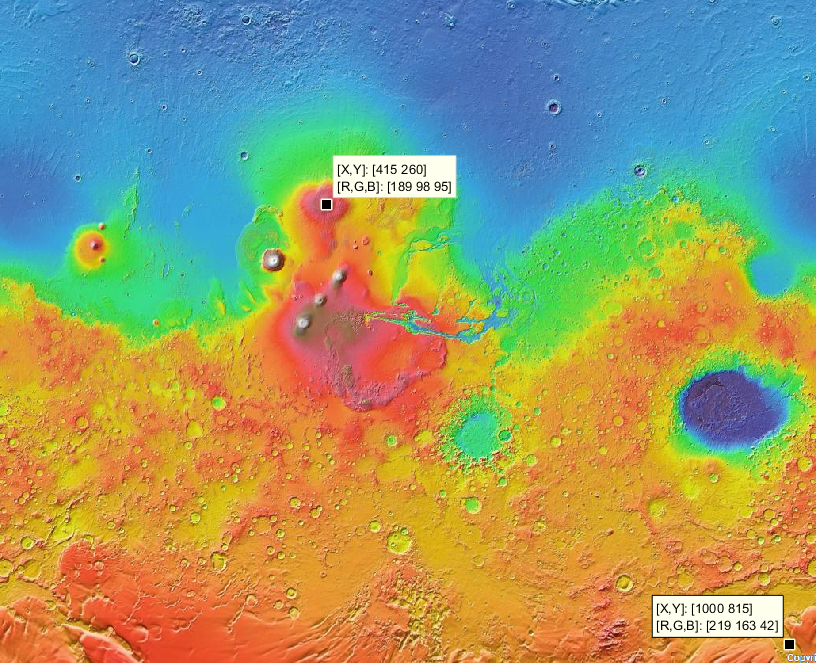
\includegraphics[width=0.5\textwidth]{mars.png}
%	\caption{Base of operations (260, 415) and supplies (815, 100).}
%	\label{fig:map}
%\end{figure}

%------------------------------------------------
\subsection{Looking for a Path}
%------------------------------------------------

Given the current position on the map, the next position is determined according to: (1) the value of the neighbouring pixels; and (2) the distance between neighbouring pixels and final destination. First calculate the Euclidean distance between all 8-neighbours of the current pixels and the destination. Then, mark as candidates the three 8-neighbours that are closest to the destination. The next position will be the candidate pixel with the lowest gray level.
\\\\
Does this algorithm produce a path between the base of operations and the supplies' landing zone? If not, suggest modifications that yield a valid outcome. Suggested modifications must include assumptions about energy consumption.
\\\\
Calculate the $D_m$ distance between the base of operations and the landing zone. Mark the path on the original RGB map. Show the result.

%------------------------------------------------
\section{Could There be Life?}
%------------------------------------------------

When you arrived at the destination, you decided to take some samples of soil for analysis. Back in the base, using a microscope the biologists discovered that there were two kinds of structures that could indicate the presence of microorganisms. Figure~\ref{fig:two}(b) shows an example. As a programmer with knowledge in image processing you were asked to write a program that counts the total number of connected components and determines how many of them have holes (do not use a built-in function that counts connected component).


%\begin{figure}[h]
%	\centering
%	\fbox{
\includegraphics[width=0.5\textwidth]{spots.png}}
%	\caption{Base of operations $MHeq(260, 415)$ and supplies $MHeq(815, 1000)$.}
%	\label{fig:microo}
%\end{figure}

\begin{figure}
	\centering
	\begin{subfigure}[b]{0.4\textwidth}
		\fbox{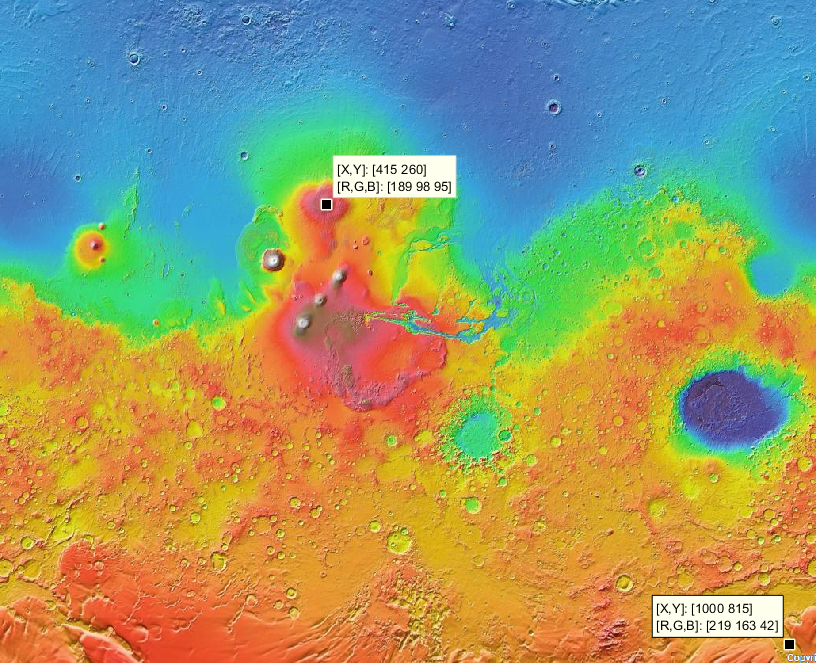
\includegraphics[height=5cm]{mars.png}}
		\caption{}
		\label{fig:mars}
	\end{subfigure}
	~ %add desired spacing between images, e. g. ~, \quad, \qquad, \hfill etc. 
	%(or a blank line to force the subfigure onto a new line)
	\hspace{3eM}
	\begin{subfigure}[b]{0.4\textwidth}
		\fbox{
\includegraphics[height=5cm]{spots.png}}
		\caption{}
		\label{fig:spots}
	\end{subfigure}
	\caption{(a) Base location and supplies landing zone; and (b) potential microorganisms.}\label{fig:animals}
	\label{fig:two}
\end{figure}


\subsection{Suggested Algorithm}


\begin{codebox}
	\Procname{$\proc{Criate-Label-Image}(I, L)$}
	\li \For $i \gets 0$ \To $\attrib{M-1}{}$
	\li \Do
 	\For $j \gets 0$ \To $\attrib{N-1}{}$
	\li \Do
	$\id{p} \gets I[i][j]$
	\li \If $(p \isequal 0)$
	\Then
	\li $\id{t} \gets I[i-1][j]$
	\li $\id{r} \gets I[i][j-1]$
    \li \If $(t \isequal 1)$ AND $(r \isequal 1)$
    \Then
    \li $\id{L[i][j]} \gets new\_label$
    \li\Else
	\If $(t \isequal 0)$ OR $(r \isequal 0)$
	\Then
	\li $\id{L[i][j]} \gets known\_label$
	\li \Else
	\If $(t \isequal 0)$ AND $(r \isequal 0)$ 
	\Then
	\li\If $same\_labels$
	\Then
	\li $\id{L[i][j]} \gets label$
	\li \Else
	\If $different\_labels$
	\li $\id{L[i][j]} \gets any\_label$
	\li $save\_label\_equivalence()$
	\End
	\End
	\End
	\End
	\End
	\End
	\End
	\li $unify\_equivalent\_labels()$
	\li \Comment 1-Background; 2 to N+1 spot label (N spots)
	\li $organize\_labels()$

\end{codebox}

Use the image in Figure~\ref{fig:debug} to analyze the algorithm.

\begin{figure}[h]
	\centering
	\fbox{
\includegraphics[width=0.5\textwidth]{debug.png}}
	\caption{Debug.}
	\label{fig:debug}
\end{figure}





\end{document}